%\subsection{Elektromyografi}
%EMG er en målemetode, som måler elektrisk aktivitet genereret af musklerne \citep{chowdhury2013}. 
%En EMG-måling dækker over et samlet antal potentialer fra måleområdet, idet der aktiveres mange muskelfibre \citep{keenan2012}. \fxnote{Ved ikke, om der skal skrives noget om, at muskelfiberne inaverers af motorneuroner, og at mængden af muskelfibre pr. motorneuron afhænger af musklen og dens funktion = det ville være godt, inddrag lidt ALS - KOMMENTAR: lige nu syntes vi ikke at der er relevant}

%Der kan anvendes to forskellige typer af EMG-målinger. Den ene er en ikke-invasiv metode, der kaldes overflade-EMG, og den anden er en invasiv metode, intramuskulær EMG \citep{chowdhury2013, keenan2012}. Hertil anvendes sidstnævnte i dette projekt. 
%Ved generel anvendelse af EMG-målinger, benyttes frekvensområdet ved $10-500~Hz$, hvorfor signaler uden for dette frekvensområde kan betegnes som støj \citep{morre2003, keenan2012}.  

%Denne metode kan påvirkes af flere artefakter, som bevægelsespåvirkning og støjpåvirkning fra elnettet ($50~Hz$) \citep{keenan2012}.
%Ligeledes kan der ved EMG-målinger fremkomme elektrisk støjpåvirkning fra omkringliggende muskler i forhold til området, der måles på. Dette betegnes som crosstalk \citep{keenan2012}. 

\subsection{Elektromyografi}
Til behandling af EMG-signalet, anvendes Muscle Sensor V3 fra Advancer Technologies, der fremover vil refereres til som 'EMG-forstærker'. Denne komponent måler en differens mellem de elektriske potentialer, der måles gennem elektroderne. EMG-forstærkeren overholder de opstillede krav, og kan anvendes direkte med mikrokontrolleren. EMG-forstærkeren består af en intrumenteringsforstærker, et passivt højpasfilter, en full-wave rectifier, et aktivt lavpasfilter og en justerbar forstærker \citep{advancertech2013}. 

En illustration af, hvordan EMG-forstærkeren behandler et inputsignal fremgår af \autoref{fig:sinussignal}.
\begin{figure}[H]
\centering
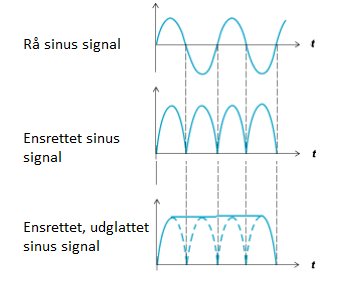
\includegraphics[width=0.6\textwidth]{figures/sinussignal.png}
\caption{Tre sinussignaler. Henholdsvis et råt, ensrettet og ensrettet samt udglattet. \citep{advancertech2013}.}
\label{fig:sinussignal}
\end{figure}

\noindent
Med udgangspunkt i \autoref{fig:sinussignal} opfattes sinuskurven som muskelsignalet. Dette passerer et passivt højpasfilter bestående af en kondensator, der dæmper DC-støjen og dermed offsettet i signalet. Dette betyder, at muskelsignalet svinger omkring tids-aksen, hvilket er nødvendigt for at få ensretningen til at virke efter hensigten. Dernæst helbølgeensrettes signalet på midterste graf, ved at invertere signalets negative værdier, så signalet udelukkende består af positive værdier samtidigt med at beholde hele dets originale energi. Herefter envelopefiltreres signalet, hvilket ses som det udglattede signal på nederste graf. Til denne filtrering er der beregnet en knækfrekvens på $1,94~Hz$ ud fra \autoref{eq:lavcutfre}. $C$ og $R$ kan i databladet for EMG-forstærkeren aflæses til at være henholdsvis $1 \cdot 10^{-6}~F$ og $80,6 \dot 10^3~\Omega$ \citep{advancertech2013}. 

% Til udglatningen er der anvendt en bin-integrator, der virker ved at beregne en middelværdi over er given stykke tid. Dette er tilsvarende at der udgregnes en middelværdi af en bestemt mængde data \citep{harb2005}. 

\begin{equation}\label{eq:lavcutfre}
f_c = \frac{1}{2 \pi C R} = \frac{1}{2 \pi \cdot 1 \cdot 10^{-6}~F \cdot 80,6 \dot 10^3~\Omega} = 1,94~Hz
\end{equation}

EMG-forstærkeren har en minimum spændingsforsyning på $\pm 3~V$ samt en maksimal spændingsforsyning på $\pm 30~V$. Herudover er der mulighed for at justere modstanden heri fra $0,1~\Omega$ til $100~k\Omega$, hvilket giver et justerbart gain fra 0,002 til 20.700 gange. \citep{advancertech2013}. 